\documentclass[pra,twocolumn,superscriptaddress,floatfix,nofootinbib,longbibliography]{revtex4-2}
\usepackage{amsfonts,amssymb,amsmath}
\usepackage{amssymb}
\usepackage{color}
\usepackage[dvipsnames]{xcolor}
\usepackage{tikz}
\usetikzlibrary{automata,arrows,positioning,calc}
\usetikzlibrary{quantikz}
\usepackage[colorlinks = true, citecolor=blue, linkcolor=blue, urlcolor=blue]{hyperref}

\begin{document}

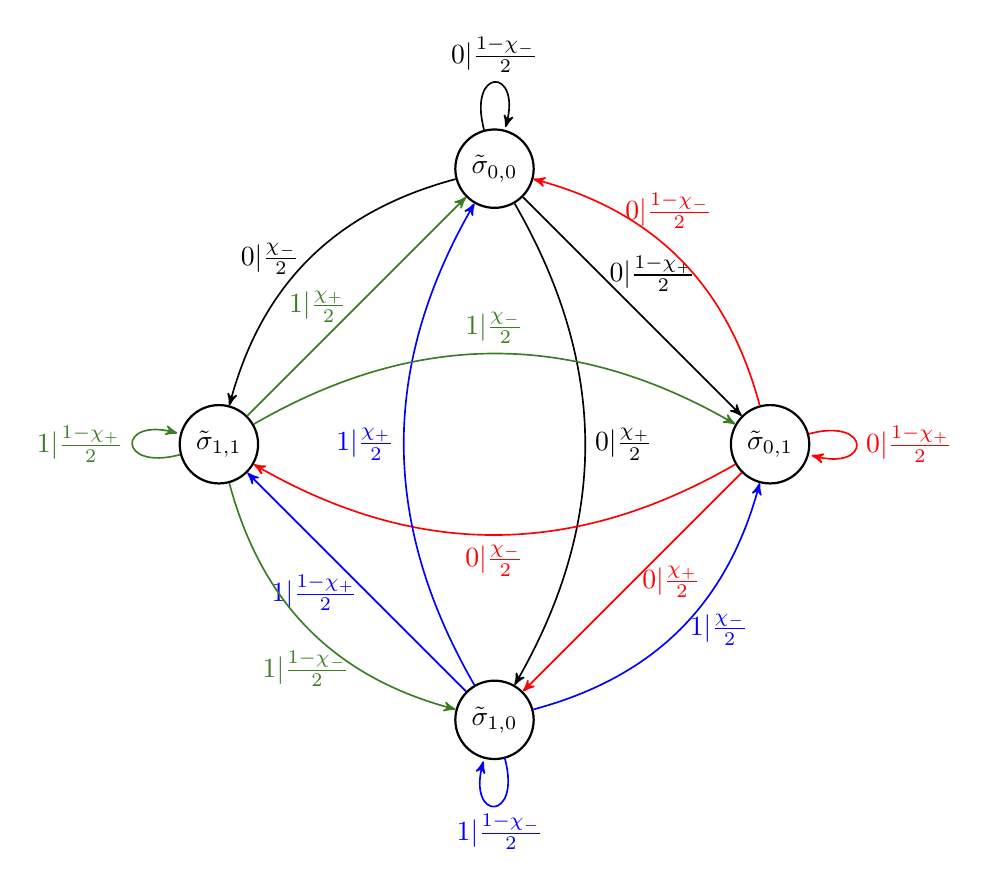
\begin{tikzpicture}[->, >=stealth', auto, semithick, node distance=3.5cm]
\tikzstyle{every state}=[fill=white,draw=black,thick,text=black,scale=1]
\node[draw=none, fill=none] (x) {};
\node[state]    (A)[above of=x]         {$\tilde{\sigma}_{0,0}$};
\node[state]    (B)[right of=x]   		{$\tilde{\sigma}_{0,1}$};
\node[state]    (C)[below of=x]         {$\tilde{\sigma}_{1,0}$};
\node[state]    (D)[left of=x]          {$\tilde{\sigma}_{1,1}$};
\path
(A) 
    edge[loop above, above] 	node{$0|\frac{1-\chi_-}{2}$}    (A)
    edge[right] 	node[pos=0.35]{$0|\frac{1-\chi_+}{2}$}    (B)
    edge[bend left, below] node[right]{$0|\frac{\chi_+}{2}$}  (C)
    edge[bend right, left] node{$0|\frac{\chi_-}{2}$}  (D)
(B)	
    edge[bend right, above, red] 	node[right,pos=0.75]{$0|\frac{1-\chi_-}{2}$}    (A)
    edge[loop right, right, red] 	node{$0|\frac{1-\chi_+}{2}$}    (B)
    edge[below, red] node[right]{$0|\frac{\chi_+}{2}$}  (C)
    edge[bend left, left, red] node[below]{$0|\frac{\chi_-}{2}$}  (D)
(C) 
    edge[bend left, above, blue] 	node[left]{$1|\frac{\chi_+}{2}$}    (A)
    edge[bend right, right, blue] 	node{$1|\frac{\chi_-}{2}$}    (B)
    edge[pos=0.4][loop below, below, blue] node{$1|\frac{1-\chi_-}{2}$}  (C)
    edge[left, blue] node[pos=0.45]{$1|\frac{1-\chi_+}{2}$}  (D)
(D) 
    edge[above, OliveGreen] 	node[left]{$1|\frac{\chi_+}{2}$}    (A)
    edge[bend left, right, OliveGreen] 	node[above]{$1|\frac{\chi_-}{2}$}    (B)
    edge[bend right, below, OliveGreen] node[left,pos=0.7]{$1|\frac{1-\chi_-}{2}$}  (C)
    edge[loop left, left, OliveGreen] node{$1|\frac{1-\chi_+}{2}$}  (D);
\end{tikzpicture}

\end{document}